\documentclass[10pt]{article}

\usepackage[margin=0.65in]{geometry}
\usepackage{amsmath,amssymb}
\usepackage{booktabs}
\usepackage{array}
\usepackage{graphicx}
\usepackage[table]{xcolor}
\usepackage{float}
\usepackage{caption}
\usepackage{subcaption}

\definecolor{taskhighlight}{HTML}{FFF2CC}
\graphicspath{{plots/}}

\setlength{\parindent}{0pt}
\setlength{\parskip}{3pt}
\setlength{\tabcolsep}{4pt}
\renewcommand{\arraystretch}{1.08}

\title{\vspace{-1.0cm}Hybrid OPD: Quick Results and Formalization}
\date{}

\begin{document}
\maketitle
\vspace{-1.1cm}

\section*{Setup}
We compare GRPO, OPD with an SFT teacher, OPD with an RL teacher, and the success-gated hybrid OPD variant. All plotted hybrid runs use gate threshold $\tau=0.0$ (\texttt{thr0p0} in the run name), so any positive trajectory reward selects the environment/GRPO branch. Plots report same-task and held-out task success over checkpoint step. When multiple seeds share the same run name except for seed, the line is the seed mean and the shaded band is a Gaussian 95\% confidence interval.

\section*{Short Absolute-Metric Table}
\begin{table}[H]
\centering
\scriptsize
\caption{Base, SFT-teacher, and GRPO step-60 absolute success metrics. The trained task column is highlighted.}
\resizebox{\linewidth}{!}{%
\begin{tabular}{>{\raggedright\arraybackslash}p{0.09\linewidth}>{\raggedright\arraybackslash}p{0.28\linewidth}*{7}{>{\centering\arraybackslash}p{0.075\linewidth}}}
\toprule
Training Task & Model & Task 0 & Task 1 & Task 2 & Task 3 & Task 4 & TRN AVG & HLD AVG \\
\midrule
task\_0 & Base & \cellcolor{taskhighlight}0.66 $\pm$ 0.02 & 0.20 $\pm$ 0.02 & 0.89 $\pm$ 0.01 & 0.65 $\pm$ 0.01 & 0.32 $\pm$ 0.02 & 0.54 $\pm$ 0.01 & 0.40 $\pm$ 0.00 \\
\midrule
task\_1 & Base & 0.66 $\pm$ 0.02 & \cellcolor{taskhighlight}0.20 $\pm$ 0.02 & 0.89 $\pm$ 0.01 & 0.65 $\pm$ 0.01 & 0.32 $\pm$ 0.02 & 0.54 $\pm$ 0.01 & 0.40 $\pm$ 0.00 \\
task\_1 & SFT teacher eval (task 1) & 0.00 & \cellcolor{taskhighlight}0.95 & 0.00 & 0.00 & 0.00 & 0.19 & 0.00 \\
task\_1 & GRPO step 60 & 0.67 & \cellcolor{taskhighlight}0.75 & 0.89 & 0.68 & 0.44 & 0.69 & 0.43 \\
\midrule
task\_4 & Base & 0.66 $\pm$ 0.02 & 0.20 $\pm$ 0.02 & 0.89 $\pm$ 0.01 & 0.65 $\pm$ 0.01 & \cellcolor{taskhighlight}0.32 $\pm$ 0.02 & 0.54 $\pm$ 0.01 & 0.40 $\pm$ 0.00 \\
task\_4 & SFT teacher eval (task 4) & 0.01 & 0.00 & 0.09 & 0.15 & \cellcolor{taskhighlight}0.87 & 0.22 & 0.02 \\
task\_4 & GRPO step 60 & 0.49 & 0.25 & 0.86 & 0.76 & \cellcolor{taskhighlight}0.77 & 0.63 & 0.43 \\
\bottomrule
\end{tabular}
}
\end{table}

\section*{Hybrid OPD Formalization}
For a trajectory $i$, define the environment success score
\[
S_i = \sum_t r_{i,t}.
\]
GRPO computes a group-relative environment advantage over group $G$:
\[
A_i^{\mathrm{env}} =
\frac{S_i - \mu_G}{\sigma_G + \epsilon},
\qquad
\mu_G = \frac{1}{|G|}\sum_{j\in G} S_j.
\]
OPD gives dense teacher feedback from teacher/student log-probability margins:
\[
m_{i,t,k} =
\log \pi_T(a_{i,t,k}\mid s_{i,t})
- \log \pi_{\theta_{\mathrm{old}}}(a_{i,t,k}\mid s_{i,t}),
\qquad
A_{i,t,k}^{T} = \mathrm{Norm}(m_{i,t,k}).
\]
The success gate uses threshold $\tau$ and teacher weight $\lambda$:
\[
g_i = \mathbf{1}[S_i > \tau],
\qquad
A_{i,t,k}^{\mathrm{hyb}}
= g_i A_i^{\mathrm{env}}
+ (1-g_i)\lambda A_{i,t,k}^{T}.
\]
In the experiments shown here, $\tau=0.0$. Thus $g_i=1$ whenever the trajectory obtains any positive environment reward, and $g_i=0$ for zero-reward failures.
The actor update uses the GRPO/PPO clipped objective:
\[
\rho_{i,t,k}(\theta)
= \exp\left(
\log \pi_\theta(a_{i,t,k}\mid s_{i,t})
- \log \pi_{\theta_{\mathrm{old}}}(a_{i,t,k}\mid s_{i,t})
\right),
\]
\[
\mathcal{L}_{\mathrm{hyb}}(\theta)
=
\mathbb{E}_{i,t,k}
\left[
\max\left(
-A_{i,t,k}^{\mathrm{hyb}}\rho_{i,t,k},
-A_{i,t,k}^{\mathrm{hyb}}
\mathrm{clip}(\rho_{i,t,k},1-\epsilon_{\ell},1+\epsilon_h)
\right)
\right].
\]
In words: successful rollouts use environment/GRPO credit; failed rollouts use SFT-teacher dense OPD credit.

\section*{Checkpoint Results}
\begin{figure}[H]
\centering
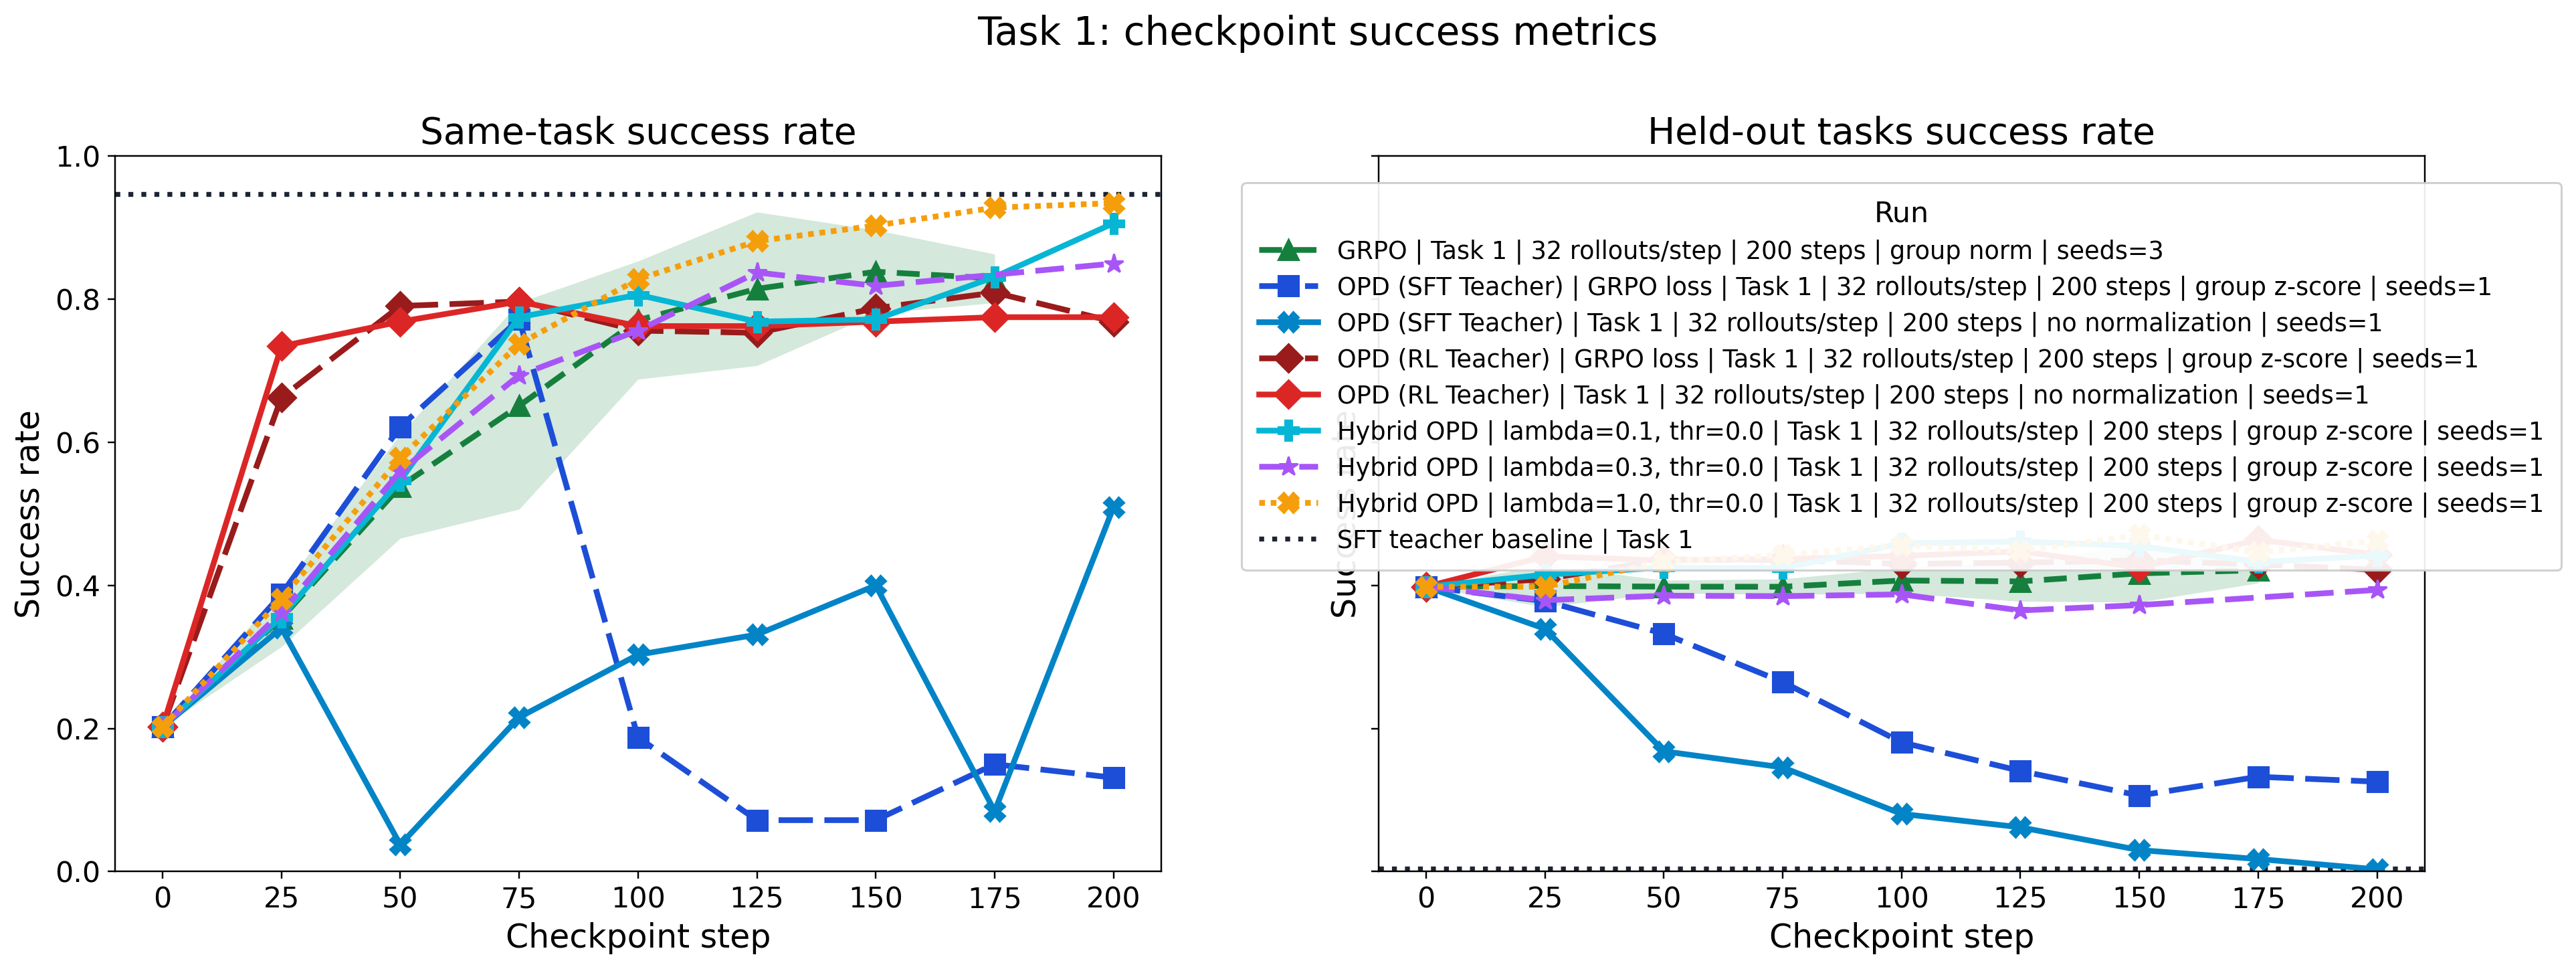
\includegraphics[width=0.94\linewidth]{rps32_task_1_checkpoint_metrics_merged.png}
\caption{rps32 comparison, Task 1. Hybrid OPD uses success-gated SFT-teacher feedback with $\lambda \in \{0.1,0.3,1.0\}$.}
\end{figure}

\begin{figure}[H]
\centering
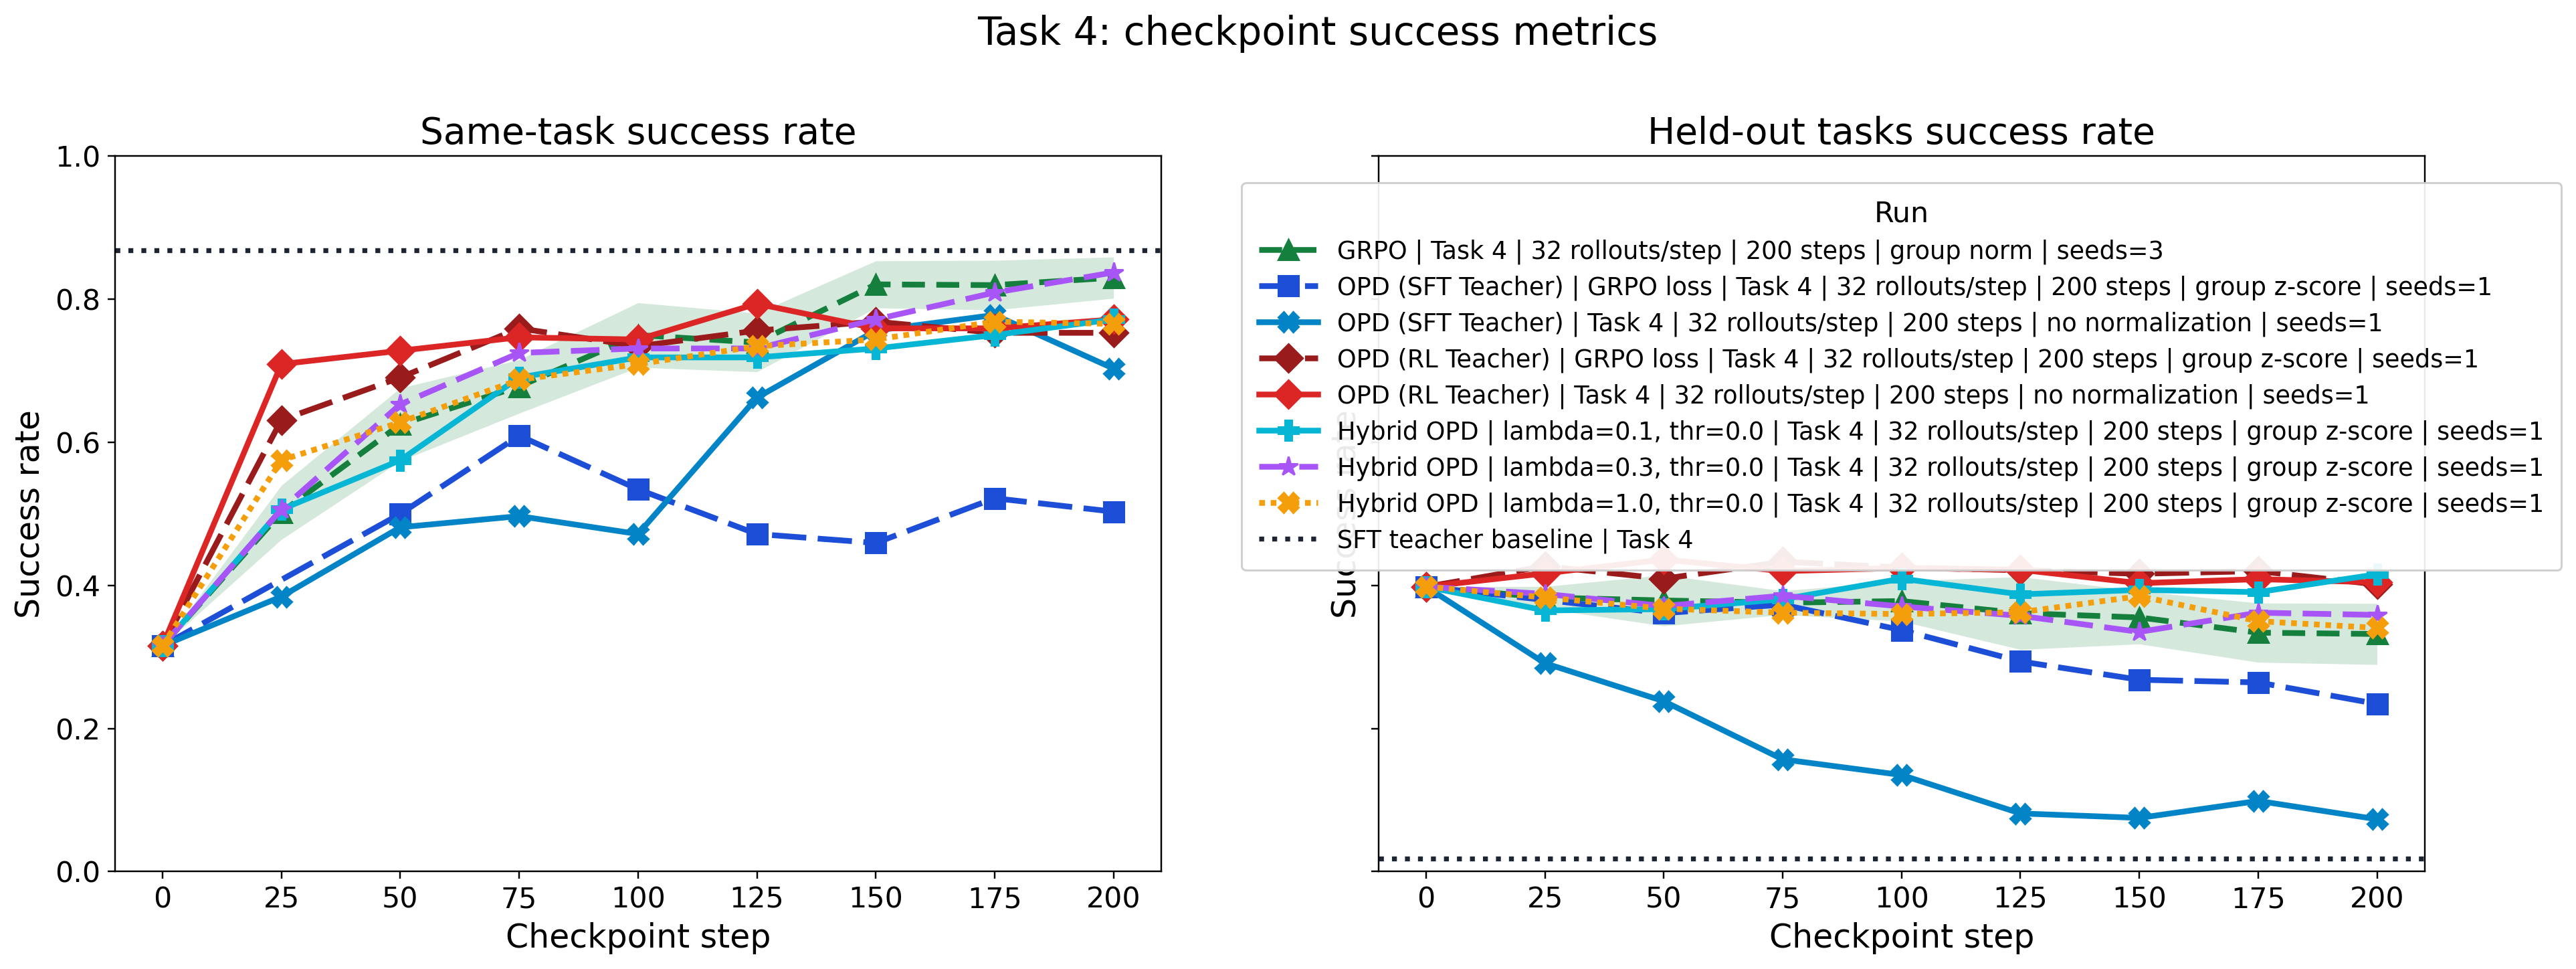
\includegraphics[width=0.94\linewidth]{rps32_task_4_checkpoint_metrics_merged.png}
\caption{rps32 comparison, Task 4. Hybrid OPD uses success-gated SFT-teacher feedback with $\lambda \in \{0.1,0.3,1.0\}$.}
\end{figure}

\begin{figure}[H]
\centering
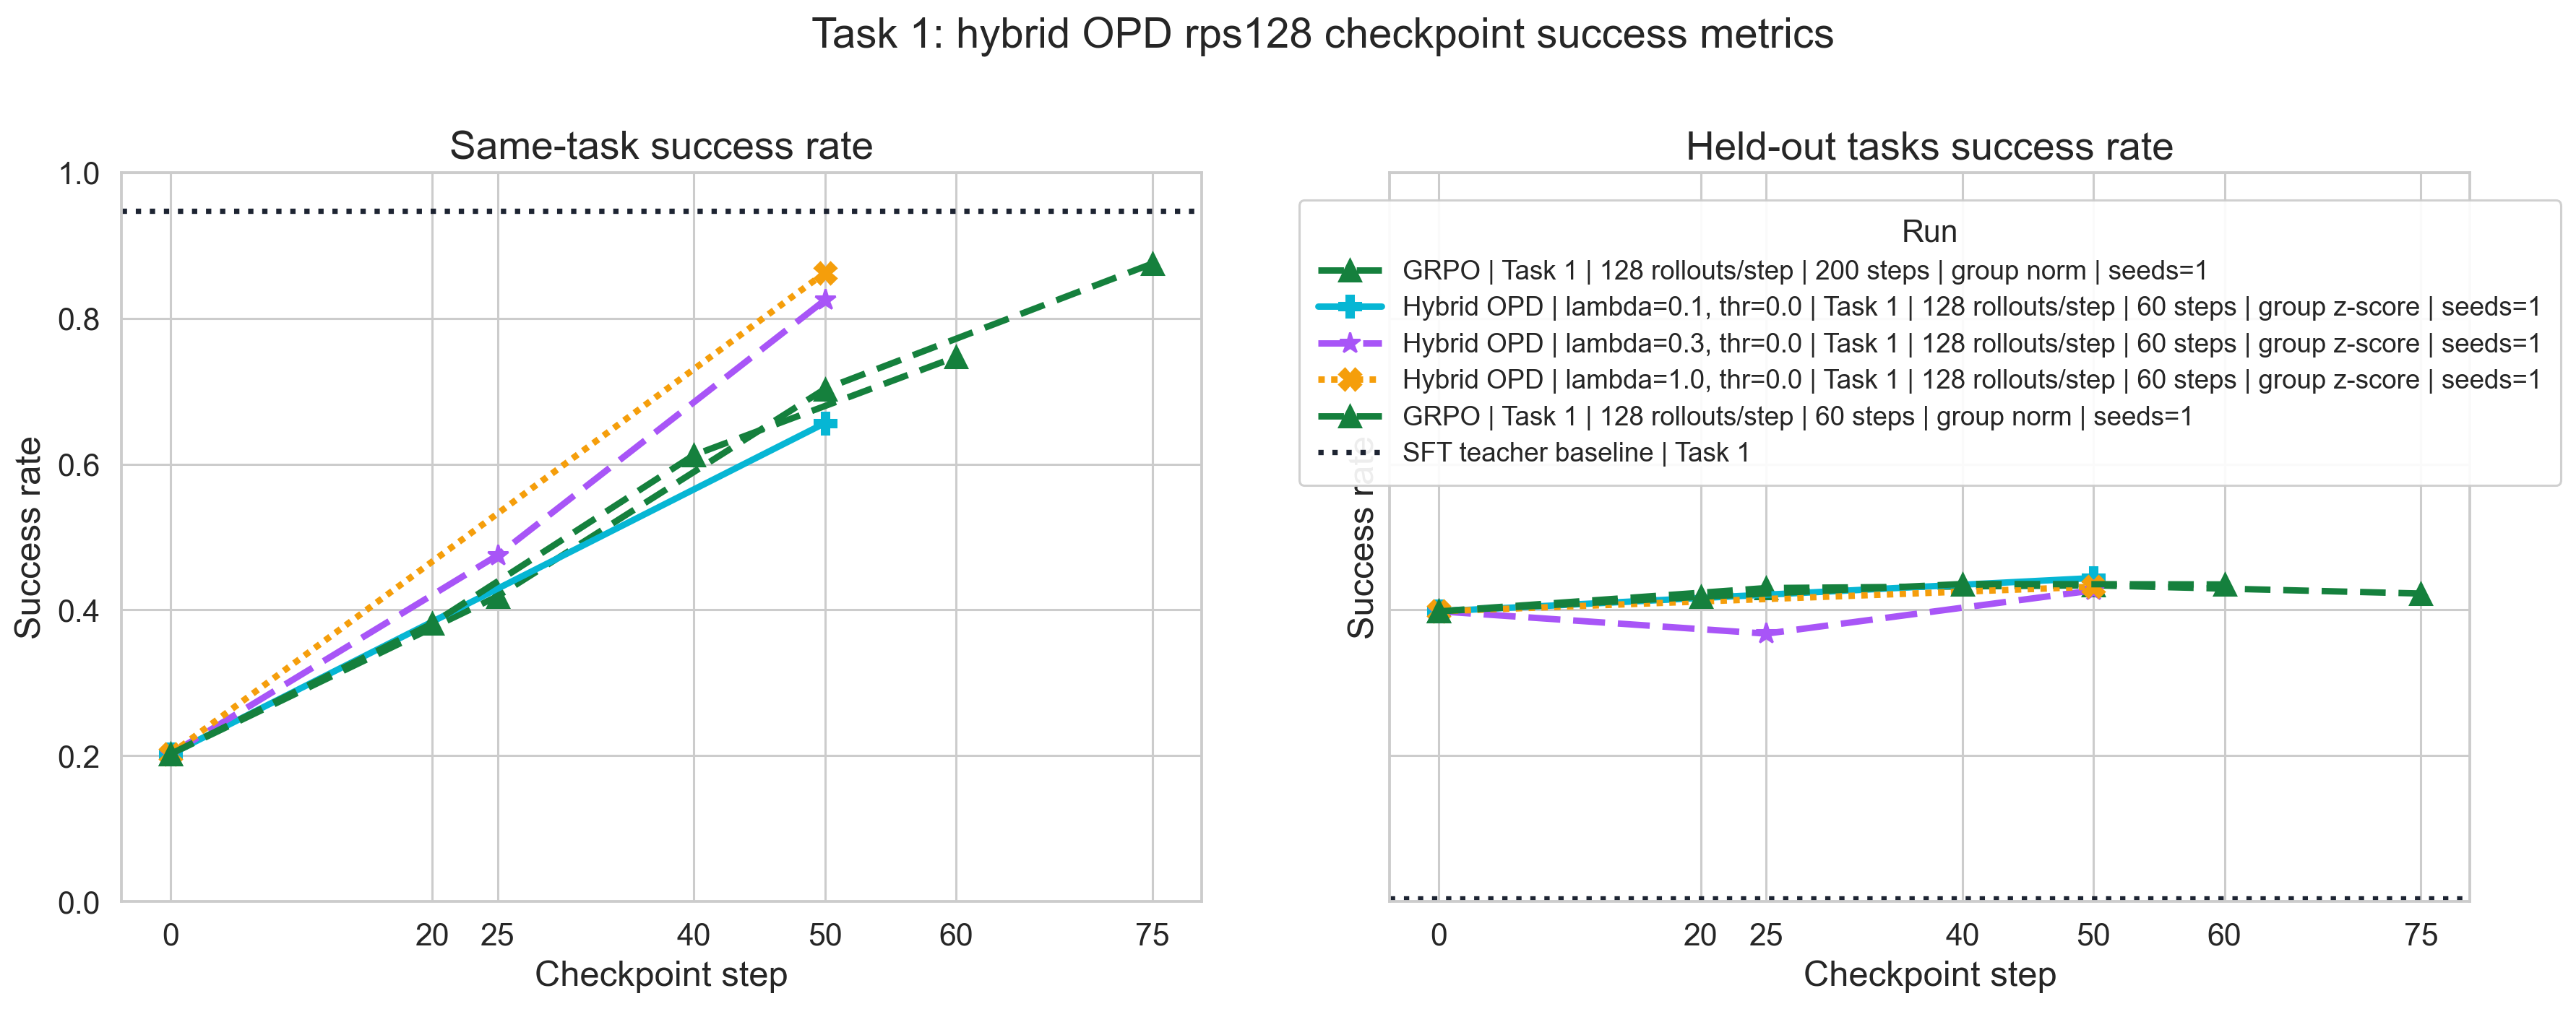
\includegraphics[width=0.94\linewidth]{rps128_success_gate_task_1_checkpoint_metrics.png}
\caption{rps128 comparison, Task 1. Kept separate from rps32 because rollout budget differs.}
\end{figure}

\begin{figure}[H]
\centering
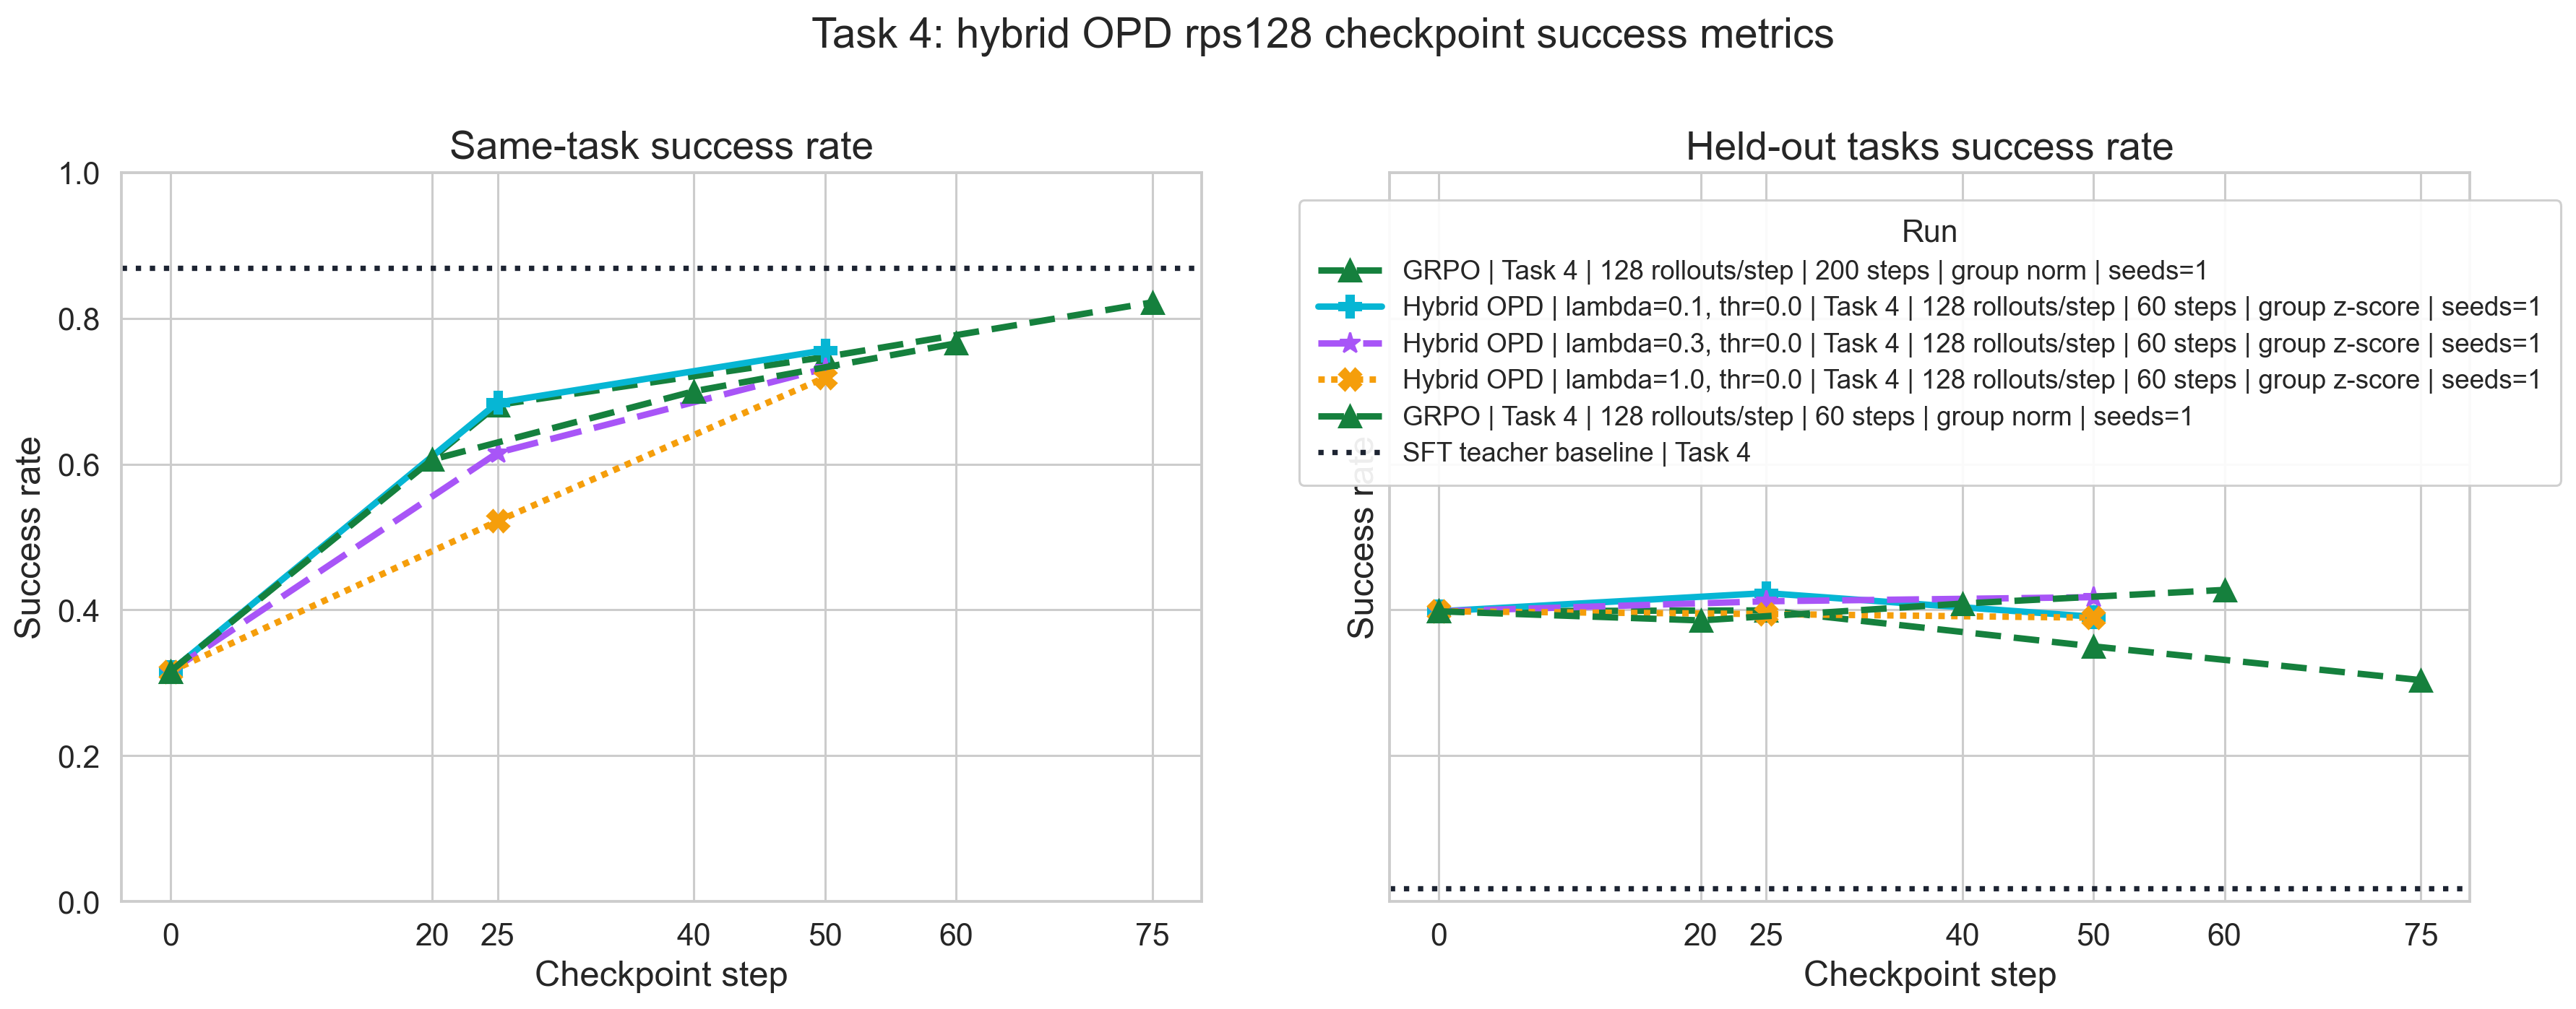
\includegraphics[width=0.94\linewidth]{rps128_success_gate_task_4_checkpoint_metrics.png}
\caption{rps128 comparison, Task 4. Kept separate from rps32 because rollout budget differs.}
\end{figure}

\section*{Takeaways}
\begin{itemize}
\item Hybrid OPD is implemented as \emph{hybrid advantages} plus the GRPO clipped policy loss.
\item The gate is simple: environment reward succeeds $\Rightarrow$ learn from GRPO signal; failure $\Rightarrow$ learn from teacher signal.
\item Current plots support quick comparison of sample efficiency and forgetting across GRPO, OPD teacher variants, and hybrid settings.
\end{itemize}

\end{document}
